\documentclass{beamer}
\usepackage{amsthm}
\usepackage{times}
\usepackage{graphicx}
\usefonttheme{professionalfonts}
\usetheme{Boadilla}
%\usecolortheme{sidebartab}
\title{Interbrain data analysis}
%\subtitle{L'equazione di Fisher}
\author[F. Bernardi]{\textbf{Fabrizio Bernardi}} \medskip
%\titlegraphic{
\includegraphics[scale=.1]{Logo_Politecnico_Milano.jpg}}
%\titlegraphic{
\includegraphics[scale=.3]{Logo_IIT.png}}





\date[02/11/2021]{02/11/2021}


\begin{document}
	
	
		\begin{frame}
	\maketitle
	
	\begin{minipage}{\linewidth}
		\centering
		\begin{minipage}{0.45\linewidth}
			\begin{figure}[H]
				
\includegraphics[width=\linewidth]{Logo_IIT.png}
				
			\end{figure}
		\end{minipage}
		\hspace{0.05\linewidth}
		\begin{minipage}{0.45\linewidth}
			\begin{figure}[H]
				
\includegraphics[width=\linewidth]{Logo_Politecnico_Milano.jpg}
				
			\end{figure}
		\end{minipage}
	\end{minipage}
\end{frame}



\begin{frame}
\frametitle{First data: observer vs stressed}





\begin{figure}[H]
	\begin{center}
		\hspace*{-1cm}
		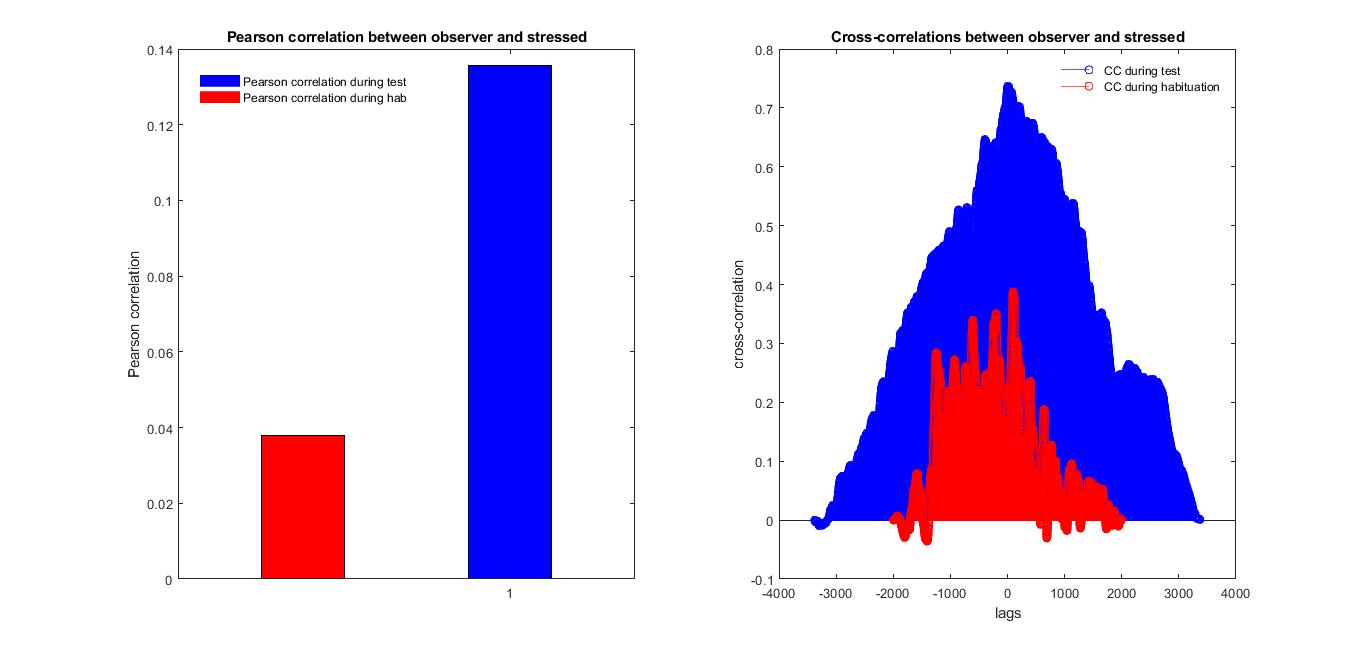
\includegraphics[scale=.30]{obs_vs_stress.jpg} 
	\end{center}  
	
	
\end{figure}


\end{frame}	

\begin{frame}
\frametitle{First data: observer vs neutral}





\begin{figure}[H]
	\begin{center}
		\hspace*{-1cm}
		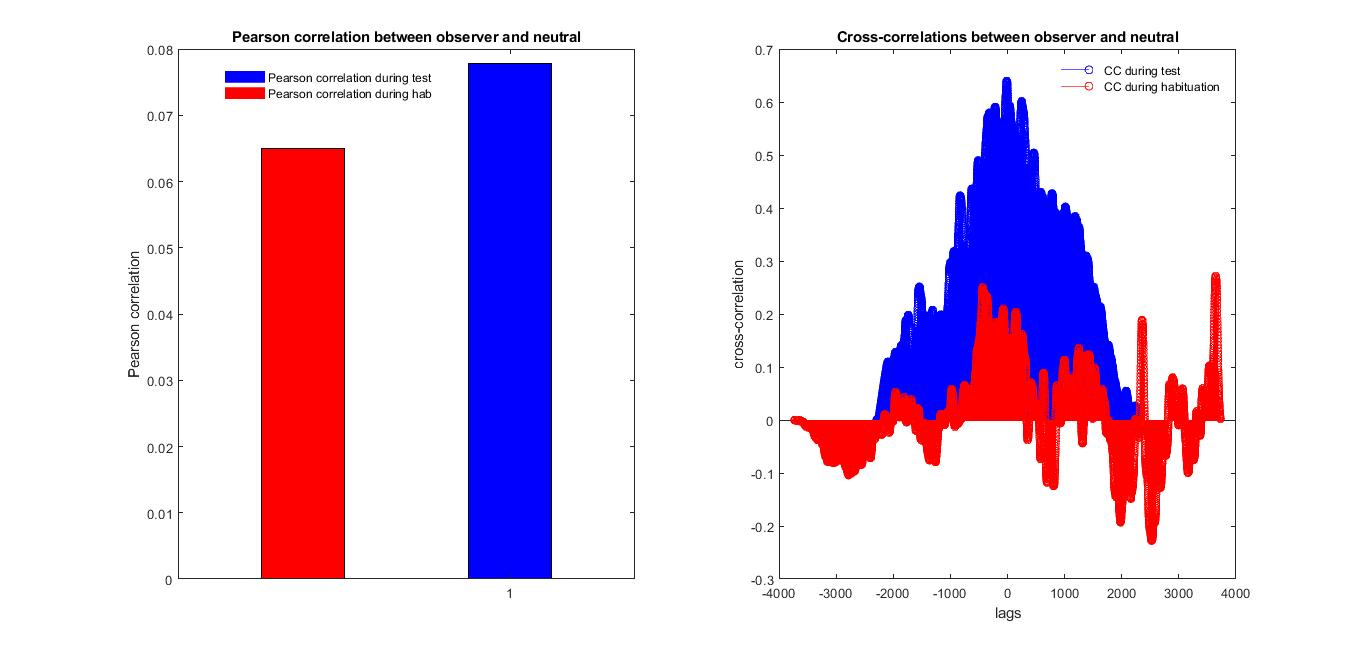
\includegraphics[scale=.30]{obs_neut.jpg} 
	\end{center}  
	
	
\end{figure}


\end{frame}	


\begin{frame}
\frametitle{First data: observer vs stressed distant }





\begin{figure}[H]
	\begin{center}
		\hspace*{-1cm}
		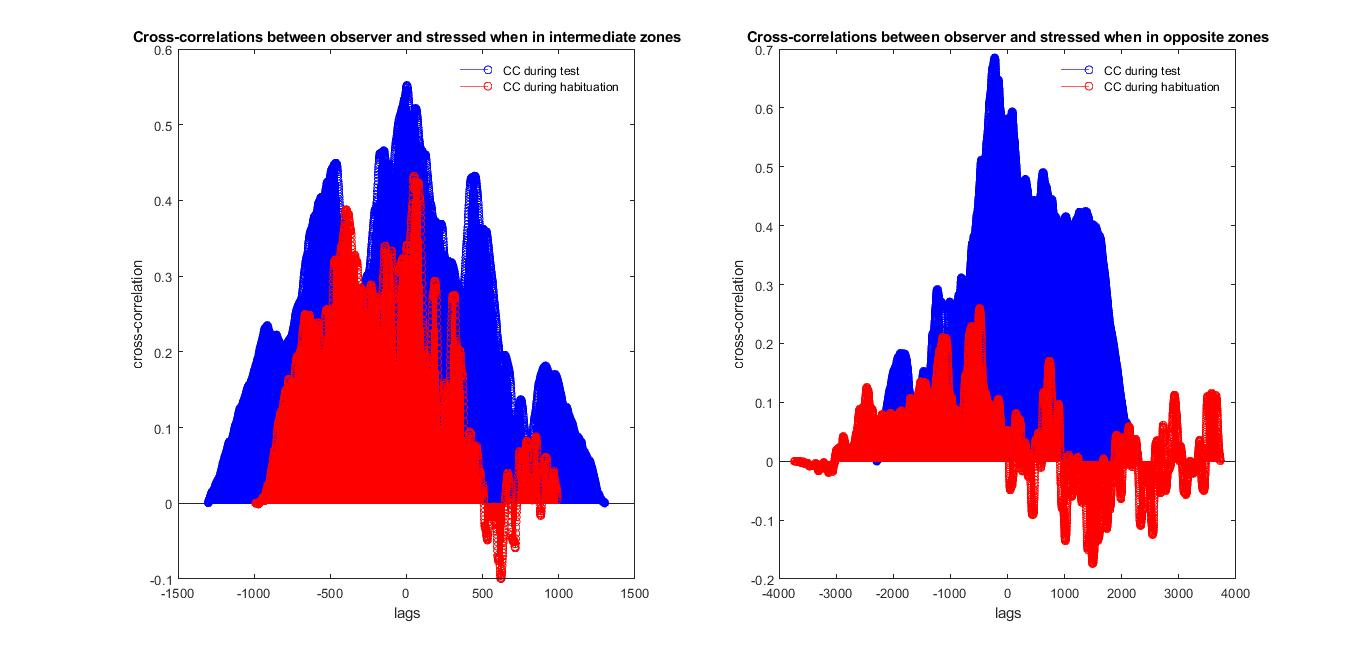
\includegraphics[scale=.30]{obs_stress_distant.jpg} 
	\end{center}  
	
	
\end{figure}


\end{frame}	


\begin{frame}
\frametitle{First data:  observer vs neutral distant}





\begin{figure}[H]
	\begin{center}
		\hspace*{-1cm}
		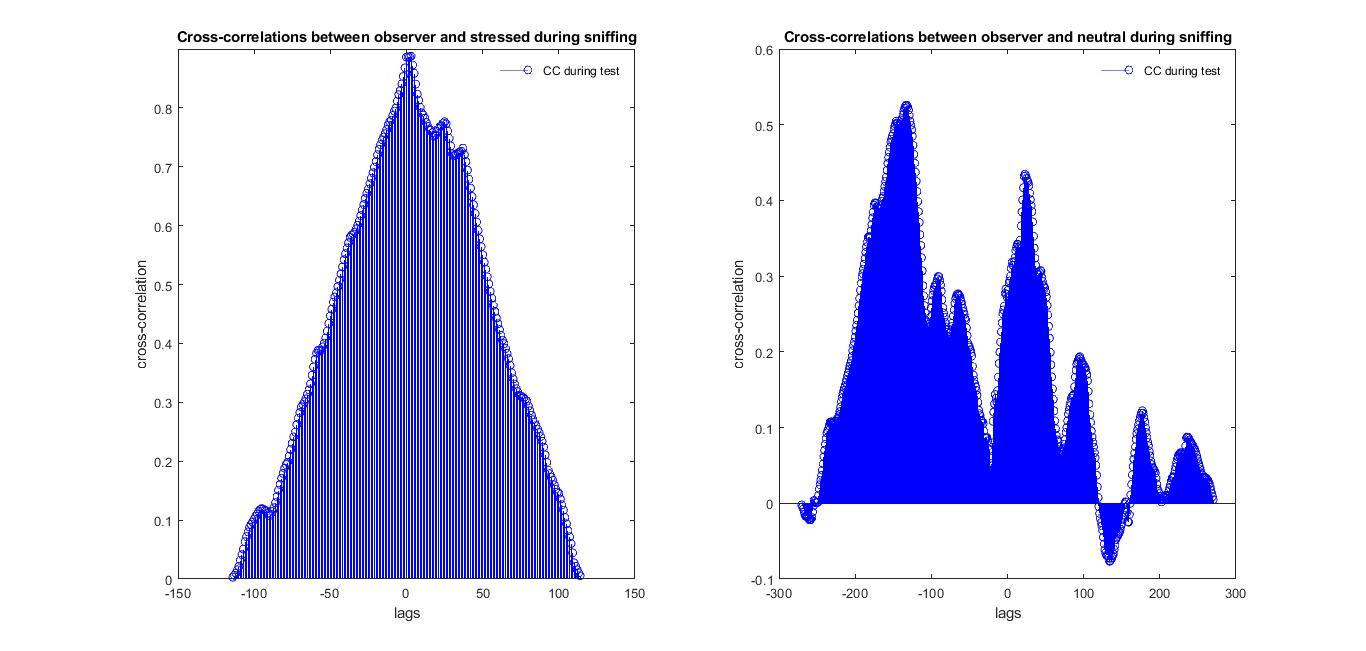
\includegraphics[scale=.30]{sniff_corr.jpg} 
	\end{center}  
	
	
\end{figure}


\end{frame}	






\begin{frame}
\frametitle{Neuron pairs synchronization: observer vs stressed during test (First data)}


Fraction of pairs showing correlation = $11.43 \%$


\begin{figure}[H]
	\begin{center}
		\hspace*{-1cm}
		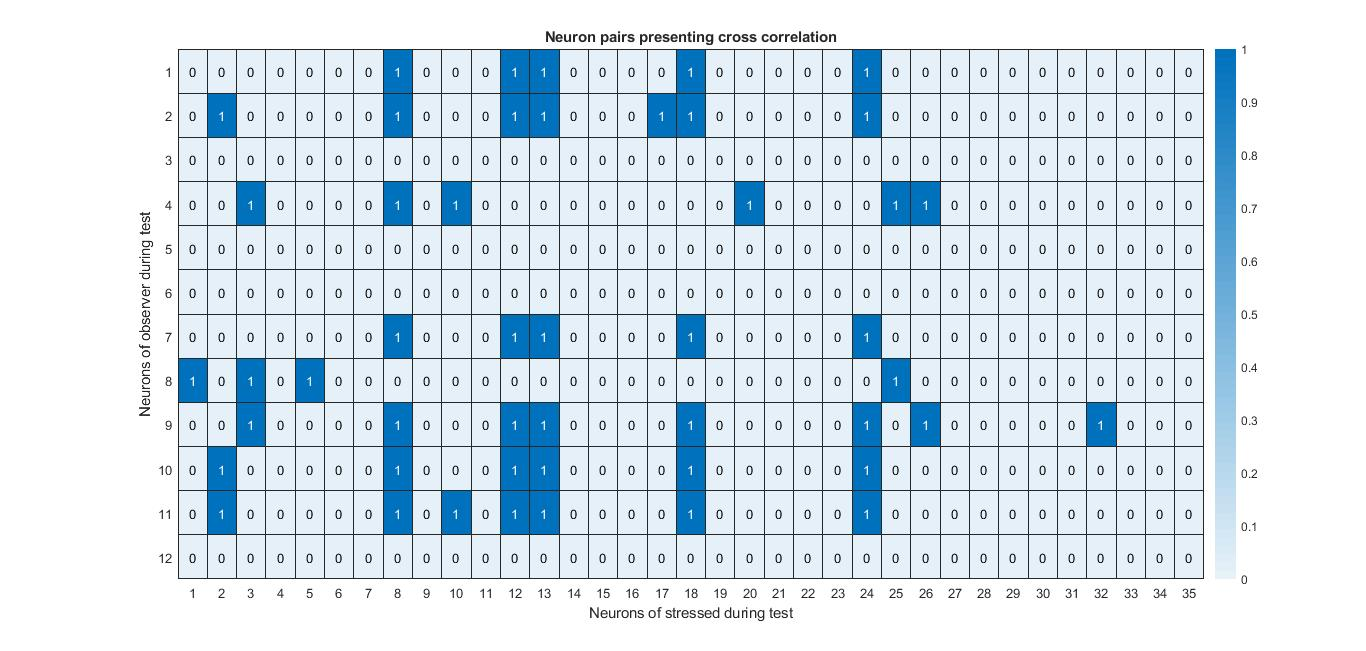
\includegraphics[scale=.30]{cc_active.jpg} 
	\end{center}  
	
	
\end{figure}


\end{frame}	






\begin{frame}
\frametitle{Neuron pairs synchronization: observer vs stressed during habituation (First data)}


Fraction of pairs showing correlation = $1.66 \%$


\begin{figure}[H]
\begin{center}
	\hspace*{-1cm}
	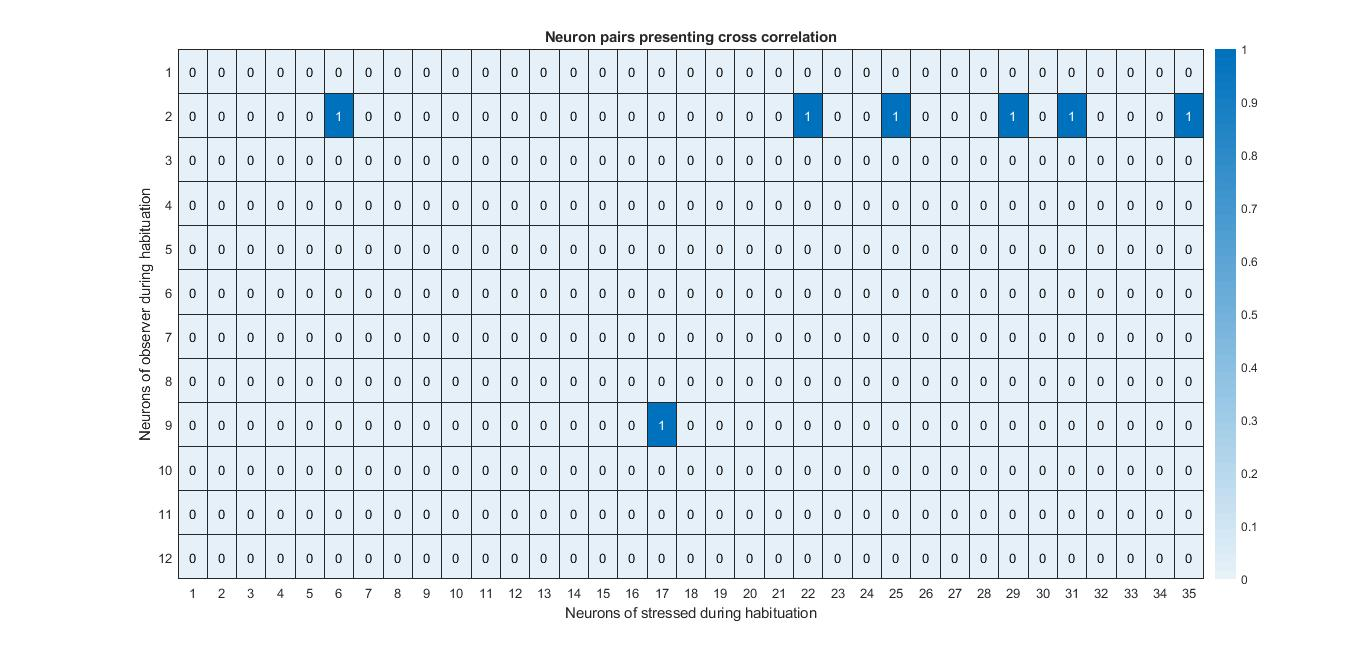
\includegraphics[scale=.30]{cc_active2.jpg} 
\end{center}  


\end{figure}


\end{frame}	







\begin{frame}
\frametitle{Neuron pairs synchronization: observer vs neutral during test (First data)}


Fraction of pairs showing correlation = $23\%$


\begin{figure}[H]
\begin{center}
	\hspace*{-1cm}
	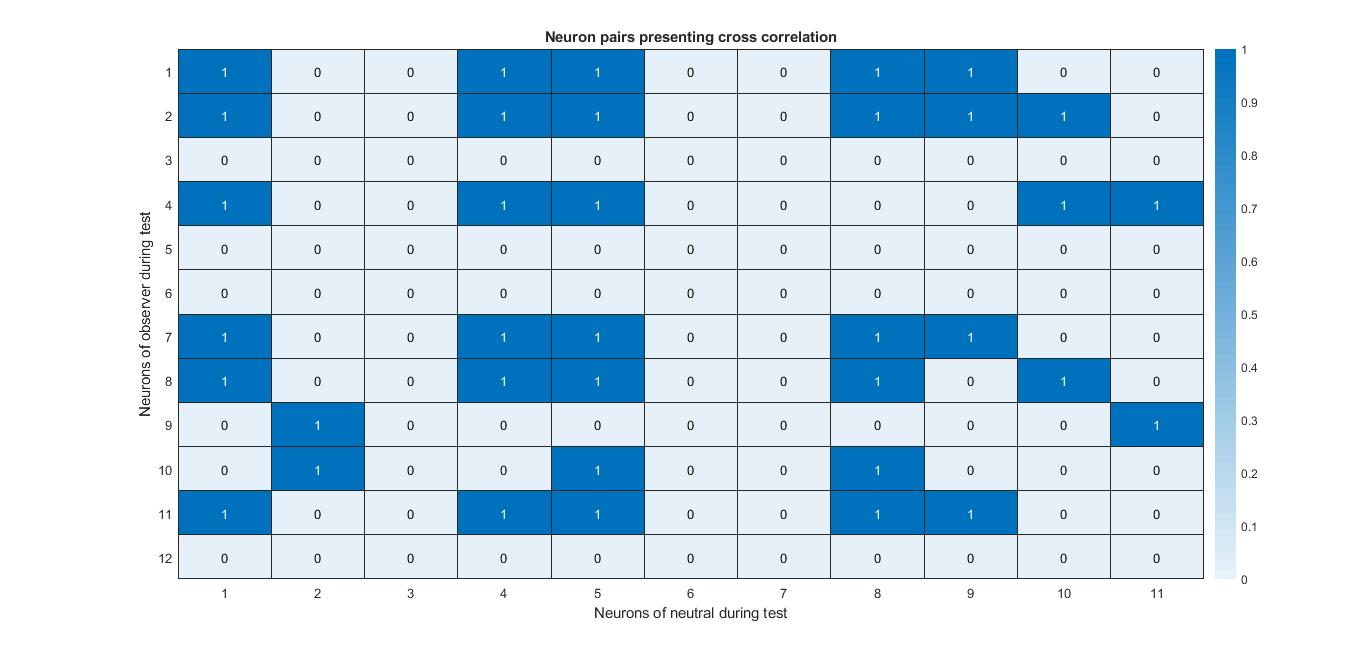
\includegraphics[scale=.30]{cc_active3.jpg} 
\end{center}  


\end{figure}


\end{frame}







\begin{frame}
\frametitle{Neuron pairs synchronization: observer vs neutral during habituation (First data)}


Fraction of pairs showing correlation = $4.5 \%$


\begin{figure}[H]
\begin{center}
	\hspace*{-1cm}
	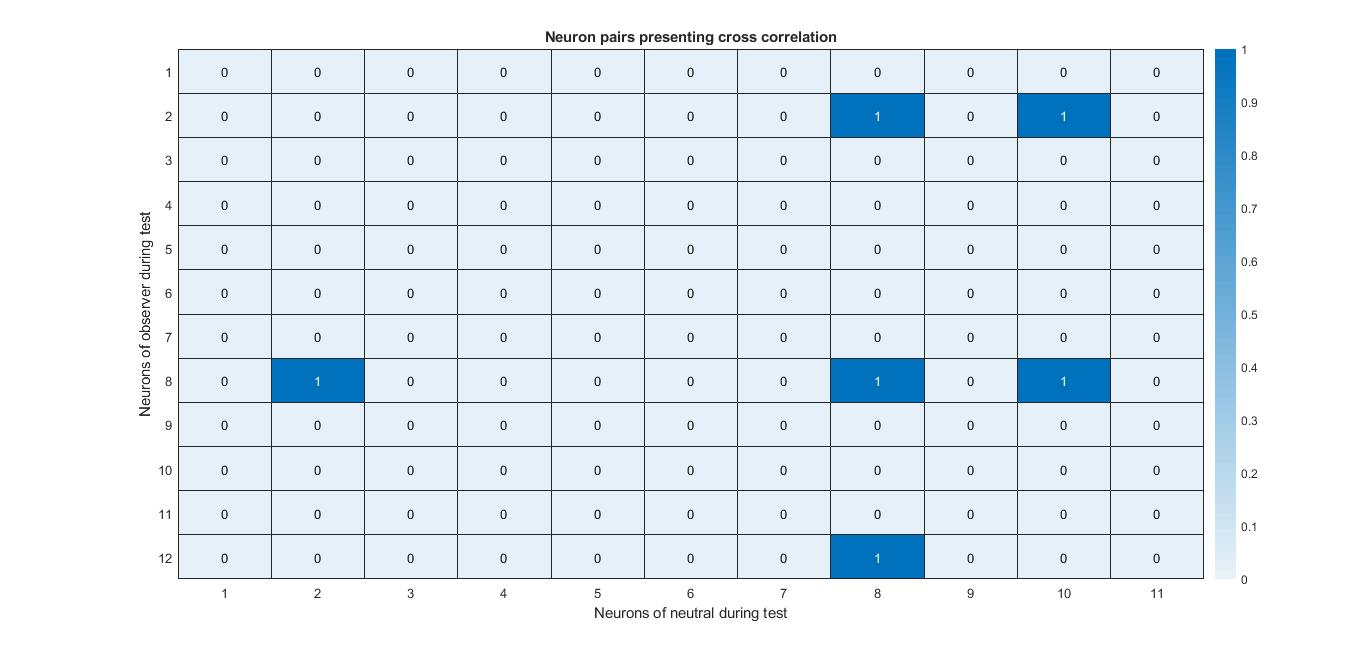
\includegraphics[scale=.30]{cc_active4.jpg} 
\end{center}  


\end{figure}


\end{frame}






\begin{frame}
\frametitle{Second data: observer vs stressed}





\begin{figure}[H]
	\begin{center}
		\hspace*{-1cm}
		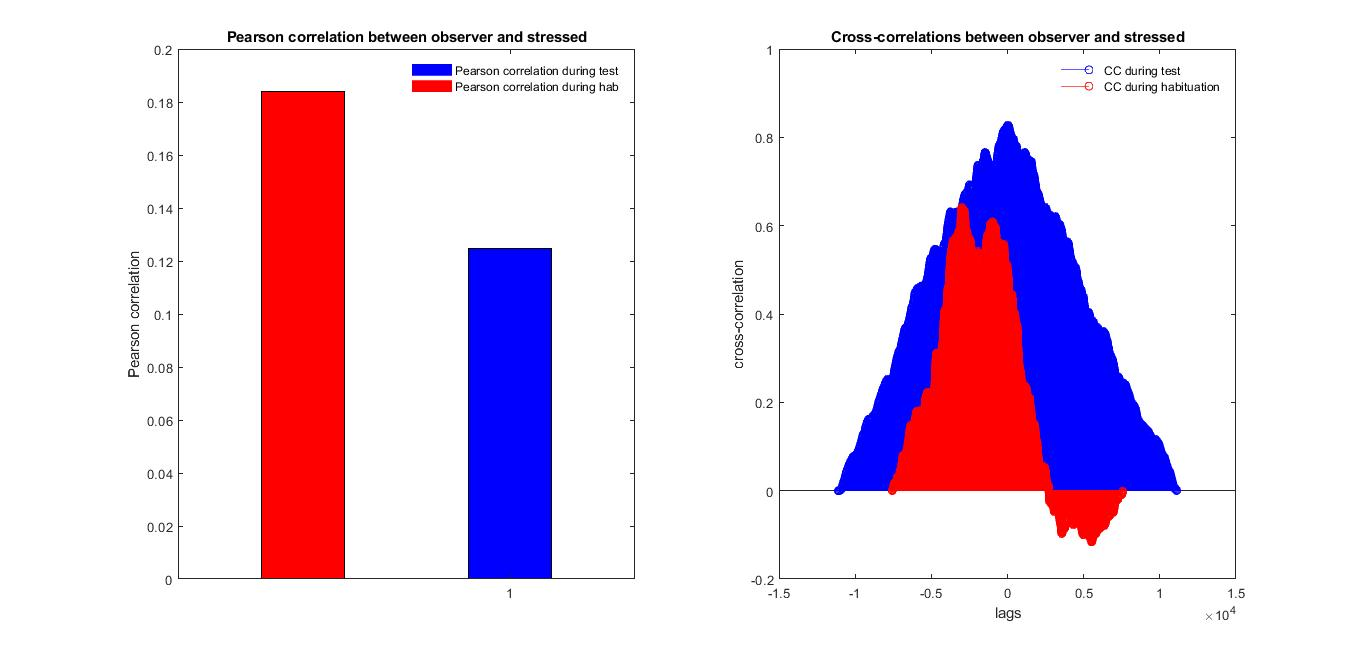
\includegraphics[scale=.30]{obs_vs_stress2.jpg} 
	\end{center}  
	
	
\end{figure}


\end{frame}	

\begin{frame}
\frametitle{Second data: observer vs neutral}





\begin{figure}[H]
\begin{center}
	\hspace*{-1cm}
	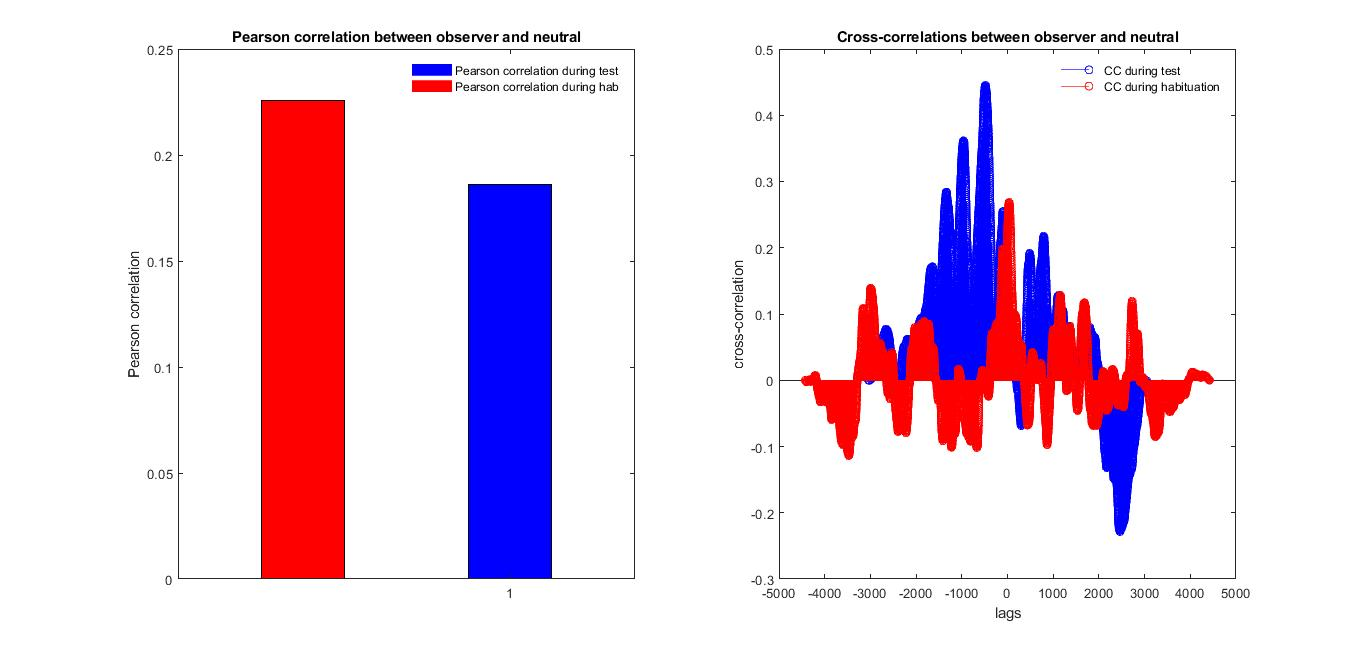
\includegraphics[scale=.30]{obs_neut2.jpg} 
\end{center}  


\end{figure}


\end{frame}	


\begin{frame}
\frametitle{Second data: observer vs stressed distant }





\begin{figure}[H]
\begin{center}
\hspace*{-1cm}
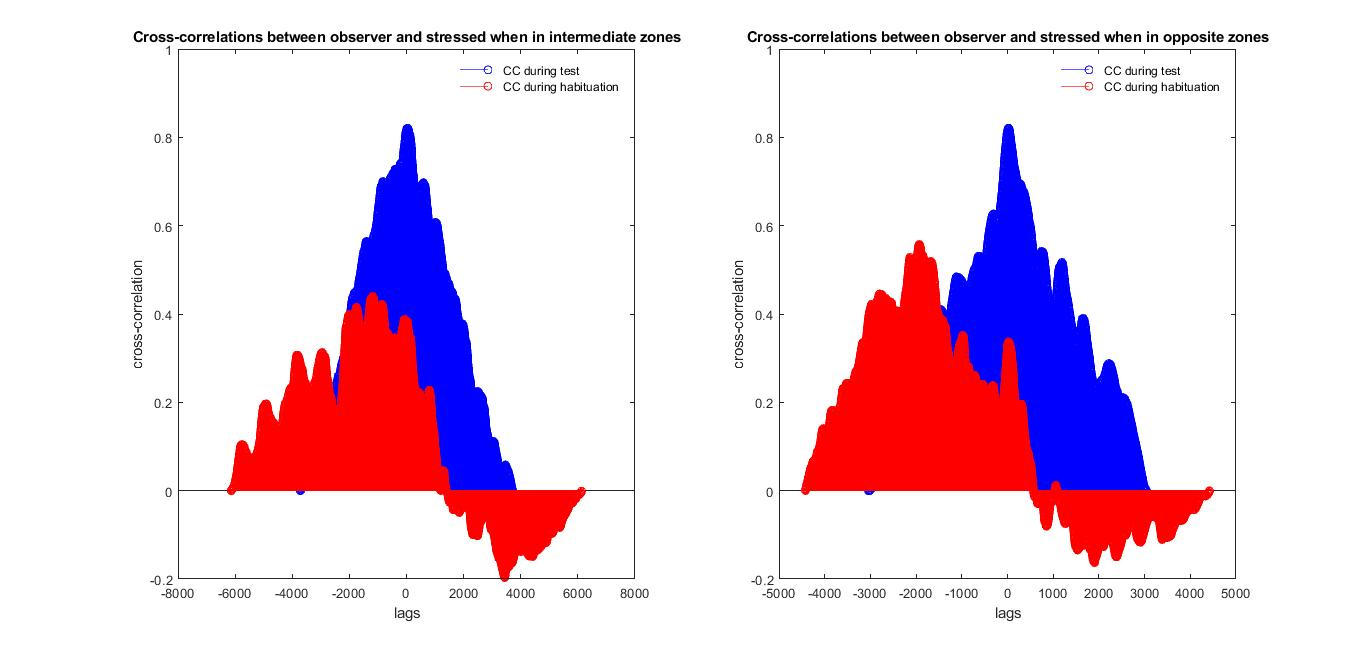
\includegraphics[scale=.30]{obs_stress_distant2.jpg} 
\end{center}  


\end{figure}


\end{frame}	


\begin{frame}
\frametitle{Second data:  observer vs neutral distant}





\begin{figure}[H]
\begin{center}
\hspace*{-1cm}
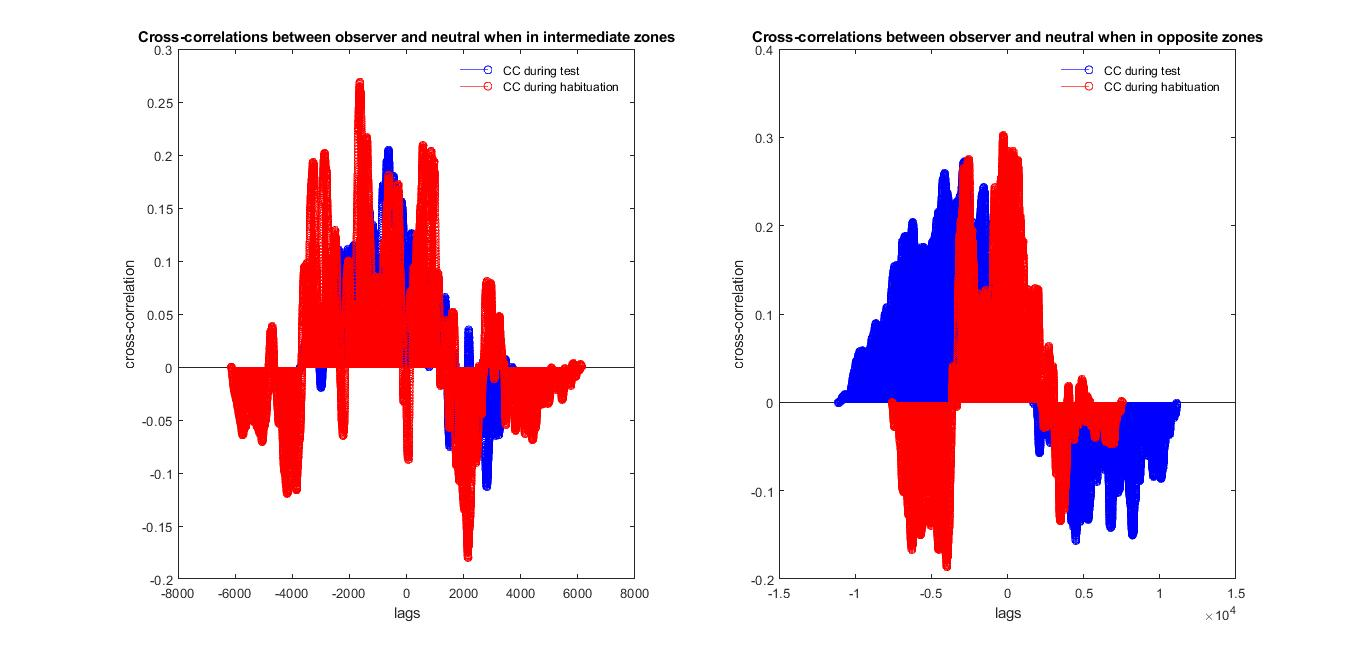
\includegraphics[scale=.30]{obs_neut_distant2.jpg} 
\end{center}  


\end{figure}


\end{frame}	

\begin{frame}
\frametitle{Second data: correlation during sniffing}





\begin{figure}[H]
	\begin{center}
		\hspace*{-1cm}
		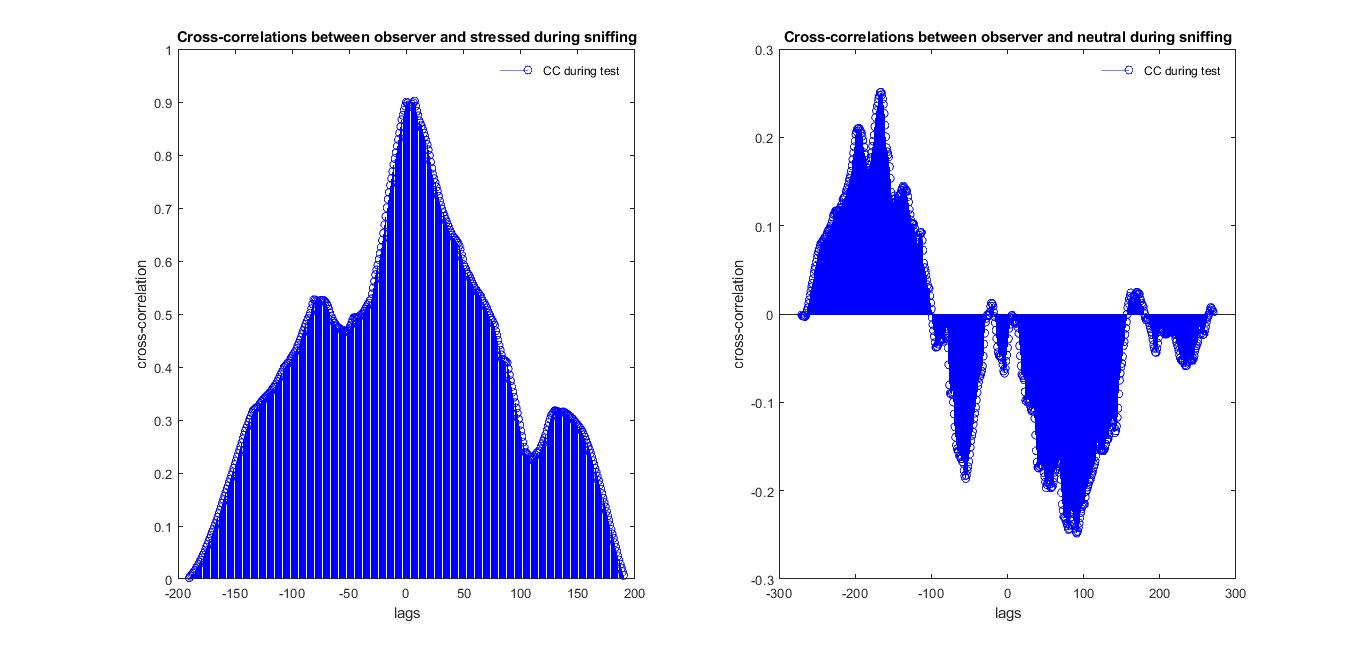
\includegraphics[scale=.30]{sniff_corr2.jpg} 
	\end{center}  
	
	
\end{figure}


\end{frame}	






\begin{frame}
\frametitle{Neuron pairs synchronization: observer vs stressed during test (Second data)}


Fraction of pairs showing correlation = $17.47 \%$


\begin{figure}[H]
\begin{center}
\hspace*{-1cm}
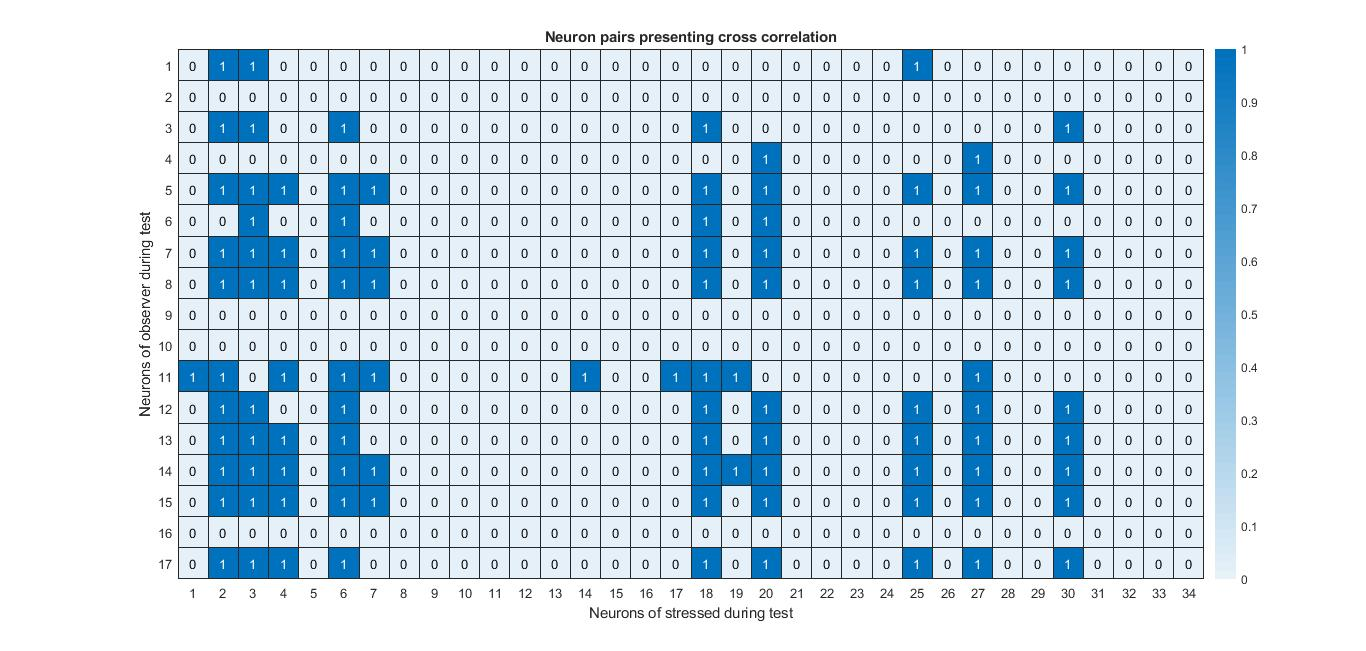
\includegraphics[scale=.30]{neur_corr_stress2.jpg} 
\end{center}  


\end{figure}


\end{frame}	






\begin{frame}
\frametitle{Neuron pairs synchronization: observer vs stressed during habituation (Second data)}


Fraction of pairs showing correlation = $1.56 \%$


\begin{figure}[H]
\begin{center}
\hspace*{-1cm}
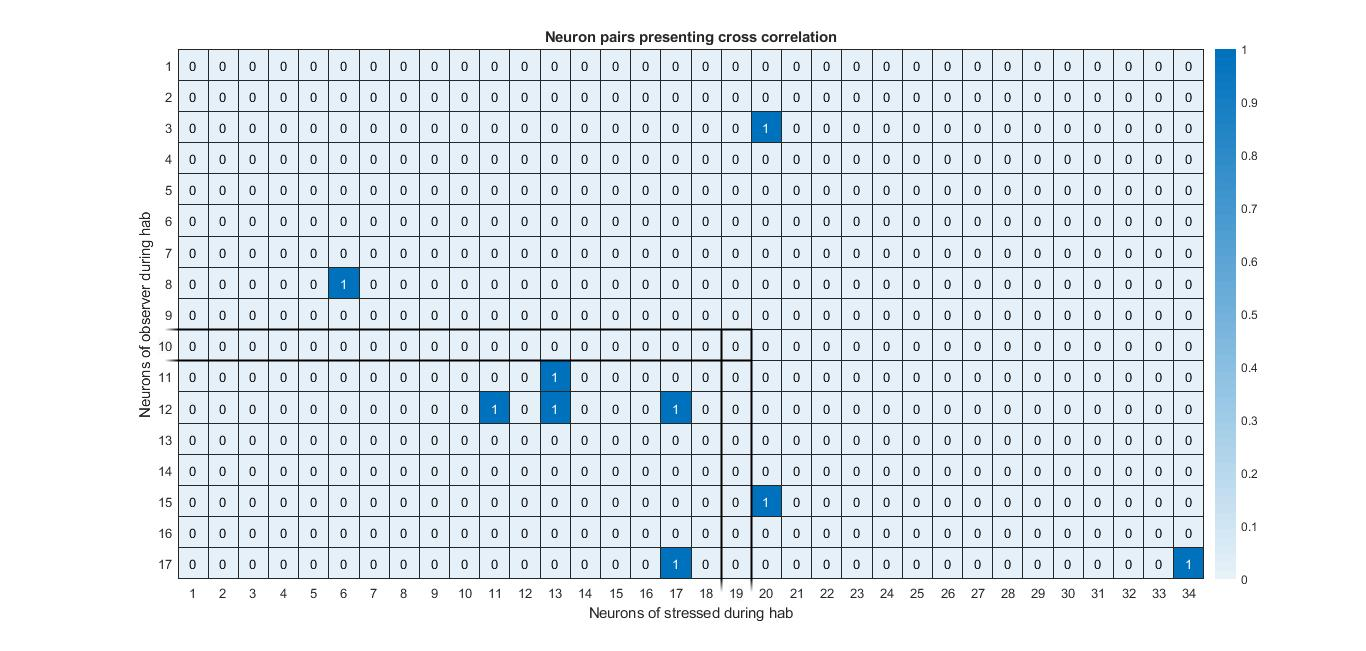
\includegraphics[scale=.30]{neur_corr_stress_hab2.jpg} 
\end{center}  


\end{figure}


\end{frame}	







\begin{frame}
\frametitle{Neuron pairs synchronization: observer vs neutral during test (Second data)}


Fraction of pairs showing correlation = $2.71\%$


\begin{figure}[H]
\begin{center}
\hspace*{-1cm}
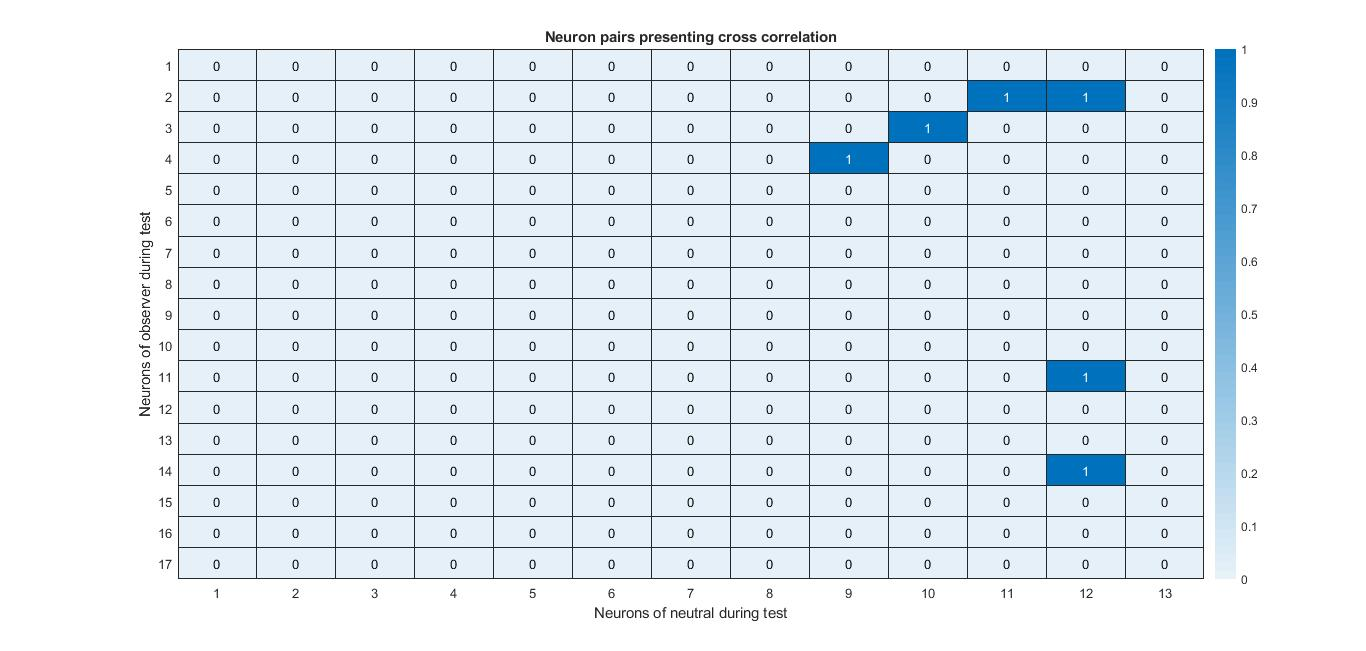
\includegraphics[scale=.30]{neur_corr_neut2.jpg} 
\end{center}  


\end{figure}


\end{frame}







\begin{frame}
\frametitle{Neuron pairs synchronization: observer vs neutral during habituation (Second data)}


Fraction of pairs showing correlation = $3.62 \%$


\begin{figure}[H]
\begin{center}
\hspace*{-1cm}
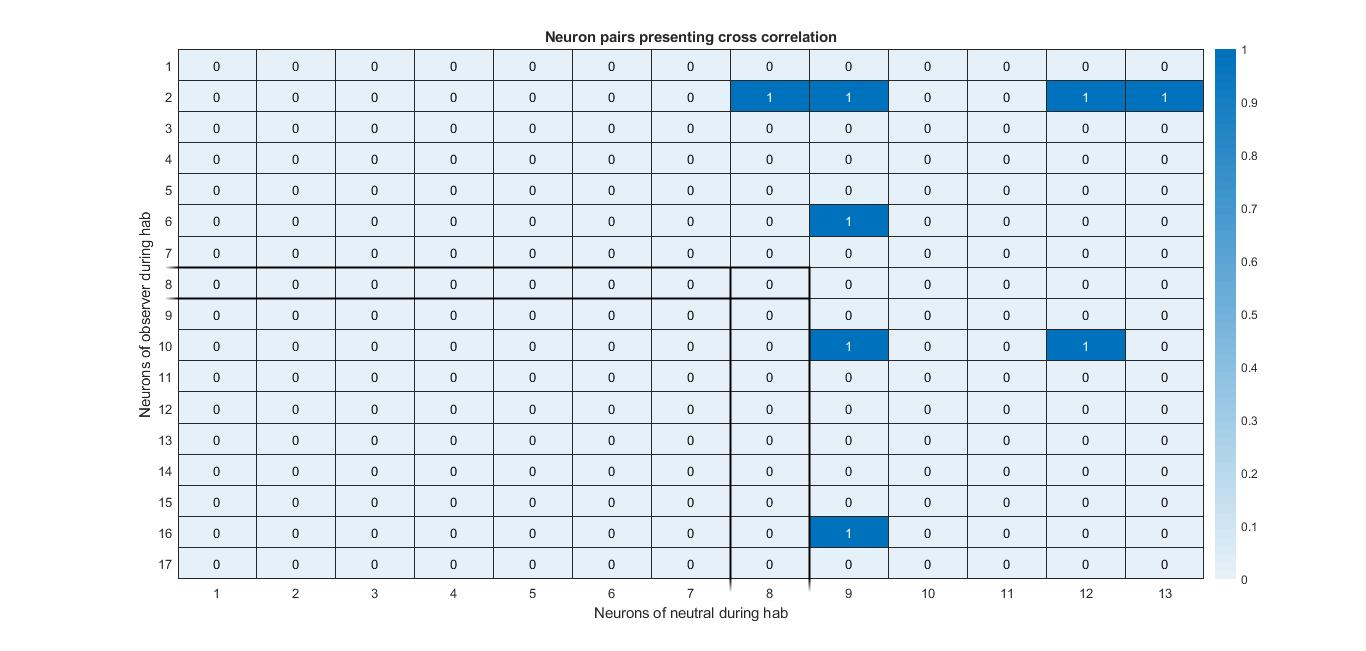
\includegraphics[scale=.30]{neur_corr_neut_hab2.jpg} 
\end{center}  


\end{figure}


\end{frame}


\begin{frame}
\frametitle{Conclusions}

\begin{itemize}
	
	\item From the first batch of data we can observe a growth in the cross correlation between mice overall activities from habituation to test, both for the pairs observer/stressed and observer/neutral, with an higher correlation in first one
	
	\item The highest correlation is observed during the sniffing between observer and stressed (but not between observer and neutral)
	
	\item In the analysis of the neuron pairs correlations we have similar results, with more pairs showing synchronization during test compared to the habituation
	
	\item As for the relationship between observer and stressed, the same results seems to appear in the second batch of data
	
	\item However, for this batch no significant correlation seems to appear between observer and neutral
\end{itemize}
\end{frame}



\end{document}

\begin{frame}
\frametitle{}
\end{frame}